%%%%%%%%%%%%%%%%%%%%%%%%%%%%%%%%%%%%%%%%%
% Simple Sectioned Essay Template
% LaTeX Template
%
% This template has been downloaded from:
% http://www.latextemplates.com
%
% Note:
% The \lipsum[#] commands throughout this template generate dummy text
% to fill the template out. These commands should all be removed when 
% writing essay content.
%
%%%%%%%%%%%%%%%%%%%%%%%%%%%%%%%%%%%%%%%%%

%----------------------------------------------------------------------------------------
%	PACKAGES AND OTHER DOCUMENT CONFIGURATIONS
%----------------------------------------------------------------------------------------

\documentclass[16pt]{article} % Default font size is 12pt, it can be changed here

\usepackage[margin=1.0in, centering]{geometry} % Required to change the page size to A4
% Set the page size to be A4 as opposed to the default US Letter

\usepackage{graphicx} % Required for including pictures
\usepackage{amsmath}
\usepackage{float} % Allows putting an [H] in \begin{figure} to specify the exact location of the figure
\usepackage{wrapfig} % Allows in-line images such as the example fish picture
\usepackage{subfigure}
\usepackage{hyperref}
\usepackage[mathscr]{euscript}
\usepackage{lipsum} % Used for inserting dummy 'Lorem ipsum' text into the template
\usepackage[english]{babel}

\usepackage{dsfont} %for fancy identity matrices \mathds{1}
\usepackage[utf8]{inputenc}
\usepackage{fancyhdr}
 
\pagestyle{fancy}
\fancyhf{}
\rhead{\textsc{Ferret} \textbf{unofficial} notes}
\lhead{UConn, ANL collaboration - [
J. Mangeri, O. Heinonen, S. Nakhmanson ]}
\rfoot{Page \thepage}


\linespread{1.5} % Line spacing

%\setlength\parindent{0pt} % Uncomment to remove all indentation from paragraphs

\begin{document}

%%----------------------------------------------------------------------------------------
%%	TITLE PAGE
%%----------------------------------------------------------------------------------------
%
%\begin{titlepage}
%
%
%\end{titlepage}

%----------------------------------------------------------------------------------------
%	TABLE OF CONTENTS
%----------------------------------------------------------------------------------------

\tableofcontents % Include a table of contents

\newpage % Begins the essay on a new page instead of on the same page as the table of contents 

%----------------------------------------------------------------------------------------
%	INTRODUCTION
%----------------------------------------------------------------------------------------

\section{Introduction}

\subsection{Elastic problem}

%
We first consider a polarizable linear elastic body, $\Omega$, under some crystallographic misfit strain, $\varepsilon_{ij}^\mathrm{misfit} (\textbf{r})$.
%
Einstein summation notation is assumed throughout this document.

Above the Curie temperature, $T_C$, the polarization, $\textbf{P}$, is zero. 
%
Thus, the total elastic free energy of the system is, 
%
\begin{equation}\tag{1}
F_\mathrm{elastic} = \int\limits_\Omega d^3 \textbf{r} \,\,\, f_\mathrm{elastic} = \int\limits_\Omega d^3 \textbf{r} \,\,\, C_{ijkl} \left(\varepsilon_{ij} - \varepsilon_{ij}^\mathrm{misfit} \right) \left(\varepsilon_{kl} - \varepsilon_{kl}^\mathrm{misfit} \right) 
\end{equation}
%
where 
%
\begin{equation}\tag{2}
\varepsilon_{ij} = \frac{1}{2} \left(\frac{\partial u_i}{\partial x_j} + \frac{\partial u_j}{\partial x_i} \right).
\end{equation}
%
Note that $u_i =  u_i (\textbf{r})$, are the displacement vectors.
%
Under mechanical equilibrium, the system obeys,
%
\begin{wrapfigure}{r}{0.5\textwidth}
  \begin{center}
\vspace{-12pt}
    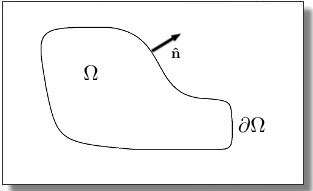
\includegraphics[width=0.475\textwidth]{geometry.jpg}
  \end{center}
  \caption{Geometry setup in \textsc{Ferret}.
%
$\Omega$ is completely bounded by surface $\partial \Omega$. $\hat{\textbf{n}}$ is an \emph{outward} facing surface normal.
%
The volume and the surface may exist as set of subdomains, $\Omega_k \subseteq \Omega_{k+1} \subseteq ... \subseteq \Omega$ and $\partial \Omega_k \subseteq \partial \Omega_{k+1} \subseteq ... \subseteq \partial \Omega$.
%
This block decomposition proves useful when defining the material properties of the problem.} %it should be noted that Moose will rename this to "subdomain" instead of block in the near future
\end{wrapfigure}
%
%
\begin{equation}\tag{3}
0 = \frac{\partial F}{\partial u_i} \Rightarrow \sigma_{ij,j} = \frac{\partial}{\partial x_j} C_{ijkl} \left(\varepsilon_{kl} - \varepsilon_{kl}^\mathrm{misfit} \right) = 0,
\end{equation}
%
the so-called stress-divergence equation \cite{Morton1975, BowerBook}.
%
The elastic stiffness tensor $C_{ijkl}$ is a rank four tensor, a 6x6 matrix, and obeys material point group symmetry \cite{NyeBook}.
%
\subsubsection{Surface elastic problem}
%
In a elastic material, a surface tension can arise from a free surface, $\partial \Omega$, bounding the body, $\Omega$.
%
Here, this surface tension, with the Gurtin-Murdoch approach \cite{Morton1975},  is related to surface tensorial quantities by
%
\begin{equation}\tag{3.1}
\sigma_{\alpha \beta}^s = \tau^0 \delta_{\alpha \beta} + C_{\alpha \beta \delta \gamma}^s \varepsilon_{\delta \gamma}^s
\end{equation}
%
where $\alpha, \beta, \gamma, \delta = 1,2$ denote crystallographic directions along the surface.
%
$C_{\alpha \beta \delta \gamma}^s$ is the surface elastic tensor, and $\varepsilon_{\delta \gamma}^s$ is a surface elastic strain. The surface elastic tensor obeys the minor symmetries $C_{\alpha \beta \gamma \delta}^s = C_{\alpha \beta \delta \gamma }^s$ and $C_{\alpha \beta \delta \gamma}^s = C_{\beta \alpha \delta \gamma }^s$ and therefore has at most nine independent components.
%
The tension, $\tau^0$ is the intrinsic surface tension.
%
A surface free energy, $F_\mathrm{surface}$ can be introduced\footnote{It should be noted that an entire \emph{module} of surface tensor mechanics could be built into the MOOSE framework based on projecting the tensorial algebra onto the surface for various pieces of physics(adsorption concentration dependent eigenstrains, surface plasticity, surface-only thermoelastic effect, ect .} as,
%
\begin{equation}\tag{3.5}
F_\mathrm{surface} = \frac{1}{2} \int\limits_{\delta \Omega} d^2 \textbf{r} \,\,\, C_{\alpha \beta \delta \gamma }^s \varepsilon_{\alpha \beta}^s \varepsilon_{\delta \gamma}^s 
\end{equation}
%
with
%
\begin{equation}\tag{3.6}
 \varepsilon_{\alpha \beta}^s = \frac{1}{2} \left(\frac{\partial u_\alpha}{\partial x_\beta} + \frac{\partial u_\beta}{\partial x_\alpha} \right).
\end{equation}
%
The purely elastic free energy balance of the volume $\Omega$ bounded by $\delta \Omega$ with body forces $\textbf{b}$ and traction $\tau$ upon the surface, under an infinitesimal displacement field $\textbf{u}$, is
%
\begin{align}\tag{3.7}
 \frac{1}{2} \int\limits_\Omega C_{ijkl} \varepsilon_{ij} \varepsilon_{kl} \,\,d^3 \textbf{r} + \frac{1}{2} \int\limits_{\delta \Omega} \,\, C_{\alpha \beta \delta \gamma}^s \varepsilon_{\alpha \beta}^s \varepsilon_{\delta \gamma}^s\,\, d^2 \textbf{r} = \int\limits_\Omega \textbf{b} \cdot \textbf{u} \,\,\,d^3 \textbf{r} + \int\limits_{\partial \Omega} \tau \cdot \mathbf{\hat{n}} \,\,d^2 \textbf{r} - \int\limits_{\partial \Omega} \tau^0_{\alpha \beta} \varepsilon_{\alpha \beta}^s \,\,d^2 \textbf{r} \\ \nonumber
\end{align}
%
for some surface normal $\mathbf{\hat{n}}$.
%
Enforcing stationary under first-order variations \cite{BowerBook}, gives us three $(k = 1,2,3)$ weak form of the equations suitable for Galerkin finite element analysis, with test function $\psi_h$:
%
\begin{align}\tag{3.8}
 0 = \int\limits_\Omega C_{ijkl} \frac{\partial u_i}{\partial x_j} \frac{\partial \psi_h}{\partial x_l} d^3 \textbf{r} + \int\limits_{\partial \Omega} C_{ijkl}^s \left(\frac{\partial u_i}{\partial x_j} \frac{\partial \psi_h}{\partial x_k} \right)_s d^2 \textbf{r} - \int\limits_\Omega b_k \psi_h d^3 \textbf{r} - \int\limits_{\partial \Omega} \tau_k \psi_h d^2 \textbf{r} + \int\limits_{\partial \Omega} \left(\tau_{ij}^0 \frac{\partial \psi_h}{\partial x_j} \right)_s d^2 \textbf{r}.
\end{align}
%
The notation $\left( . \right)_s$ denotes the projection of the tensor onto the surface.
%
These quantities are constructed and each quadrature point on the surface by taking their bulk counterparts and using a local projection operator $\mathbf{\hat{\textbf{P}}} = \mathds{1} - \mathbf{\hat{n}}(\textbf{r}) \otimes \mathbf{\hat{n}} (\textbf{r})$ \cite{Yvonnet2012} such that 
%
\begin{align}\tag{3.9}
\sigma^s = \mathbf{\hat{\textbf{P}}} \sigma \mathbf{\hat{\textbf{P}}} \,\,\,\mathrm{and}\,\,\, \varepsilon^s = \mathbf{\hat{\textbf{P}}} \varepsilon \mathbf{\hat{\textbf{P}}}.
\end{align}
%
For application of this technique, see Influence of Elastic and Surface Strains on the Optical Properties of Semiconducting Core-Shell Nanoparticles,
John Mangeri, Olle Heinonen, Dmitry Karpeyev, and Serge Nakhmanson, Phys. Rev. Applied 4, 014001 -- \href{http://journals.aps.org/prapplied/abstract/10.1103/PhysRevApplied.4.014001}{Published}  7 July 2015. 
%

%
\subsection{Ferroelectric materials below $T_C$}
%
In a ferroelectric, below the Curie temperature, spontaneous polarization arises \cite{LinesBook, RabeBook}.
%
To find a free energy description, that includes the new primary order parameter polarization, one can expand the free energy in $P_k$ and $\varepsilon_{ij}$, about $P_k = 0$, and $\varepsilon_{ij} =  \varepsilon_{ij}^\mathrm{misfit}$.
%
Here, it is assumed that $\varepsilon_{ij}^\mathrm{misfit}$ is constant in space. 
%
\begin{align}\tag{4}\label{eqn:Landau}\nonumber
F =&\int f_\mathrm{elastic} \,d^3 \textbf{r} + \frac{1}{2!}\int \frac{\delta^2 {\mathcal F}}{\delta P_i\delta P_j}P_i P_j\,d^3 \textbf{r}
+ ... + \frac{1}{4!}\int \frac{\delta^4 {\mathcal F}}{\delta P_i\delta P_j \delta P_k \delta P_l}
P_iP_jP_kP_l\, d^3 \textbf{r}\nonumber\\
+ &... +  \frac{1}{6!}\int \frac{\delta^6 {\mathcal F}}{\delta P_i\delta P_j \delta P_k \delta P_l\delta P_m \delta P_n}
P_iP_jP_kP_lP_m P_n\,d^3 \textbf{r} + ... \nonumber\\
+& \frac{1}{2}\int \frac{\delta {\mathcal F}}
{
\delta\left(\frac{\partial P_i}{\partial x_j}\right)
\delta\left(\frac{\partial P_k}{\partial x_l}\right)
}
\frac{\partial P_i}{\partial x_j}\frac{\partial P_k}{\partial x_l}\,dv-\int P_iE_i\,d^3 \textbf{r} + ...\nonumber\\
+& \frac{1}{3!}\int \frac{\delta^3 {\mathcal F}}{\delta \varepsilon_{ij}\delta P_k\delta P_l}
\left(\varepsilon_{ij}-\varepsilon_{ij}^\mathrm{misfit}\right)P_kP_l\,d^3 \textbf{r} +... \\ \nonumber
\end{align}\nonumber
%fix!%
%
Here, the higher order and mixing terms are neglected.
%
Also, ${\mathbf E} = - \nabla \Phi$ is the {\em total} electrostatic field, that is introduced into the problem to coupled to electrostatic potential, $\Phi$, due to the dipole moments \emph{and} external fields.
%
The multiderivative terms are the coefficient tensors of the expansion. We can rewrite Eq. (4) as
%
\begin{align}\tag{5}\label{eqn:Landau}
F = \int\limits_\Omega \,\, f \,\,d^3 \textbf{r} = \int\limits_\Omega \,\, \left( f_\mathrm{elastic} + f_\mathrm{bulk} + f_\mathrm{wall} + f_\mathrm{electrostatic} + f_\mathrm{coupled} \right) d^3 \textbf{r} 
\end{align}
%
with
%
\begin{equation}\tag{6}
f_\mathrm{bulk} \equiv \alpha_{ij} P_i P_j + \beta_{ijk} P_i P_j P_k + \gamma_{ijkl} P_i P_j P_k P_l + \omega_{ijklm} P_i P_j P_k P_l P_m + \delta_{ijklmn} P_i P_j P_k P_l P_m P_n,
\end{equation}
%
\begin{equation}\tag{7}
f_\mathrm{wall} \equiv  G_{ijkl} \frac{\partial P_i}{\partial x_j} \frac{\partial P_k}{\partial x_l},
\end{equation}
%
\begin{equation}\tag{8}
f_\mathrm{electrostatic} \equiv - P_k \frac{\partial \Phi}{\partial x_k},
\end{equation}
%
and 
%
\begin{equation}\tag{9}
f_\mathrm{coupled} \equiv \frac{1}{2} q_{ijkl} \left(\varepsilon_{ij} - \varepsilon_{ij}^\mathrm{misfit} \right)P_k P_l.
\end{equation}
%
The coefficient tensors, $\alpha_{ij}$, $\beta_{ijk}$, $\gamma_{ijkl}$, $\omega_{ijklm}$, $\delta_{ijklmn}$, $G_{ijkl}$, and $q_{ijkl} \equiv 2 \, C_{ijmn} Q_{mnkl}$, are material dependent, obey symmetries of the lattice, and can be dependent at temperature, $T$.
%
In general, one can use group theoretical methods \cite{WootenBook} to immediately reduce the number of terms in the expansions.
%
\section{Gradient-flow approach}
%
%To derive the time-dependent Landau-Ginzburg equations, one can follow the work in Su and Landis where we can start from a inequality of thermodynamics. This is interesting and should be done out.
%
\textsc{Ferret} is a code-package \cite{FerretLink} for the multi-physics framework MOOSE \cite{Gaston2009} which is built upon the finite element library \textsc{libMesh} \cite{Kirk2006}.
%
We aim to simulate isothermal ferroelectric nanostructures by evolving \cite{Su2007} the system energy through a time-dependent Landau-Ginzburg-Devonshire (TDLGD) equation, also known as an Allen-Cahn equation \cite{Tonks2012},
%
\begin{equation}\tag{10}
- \gamma \frac{\partial \textbf{P}}{\partial t} =  \frac{\delta}{\delta \textbf{P}}\int\limits_\Omega d^3 \textbf{r} \,\,\,f\left(\textbf{P} \right).
\end{equation}
%
Here $\gamma$ is a time-scaling parameter related to domain-wall mobility.
%
Since there is a coupling to the local strain and polar fields, the full time-dependent Ginzburg-Landau equations are
%
\begin{align}\tag{11}\label{eqn:tdGLP}
-\gamma_P\frac{\partial P_i}{\partial t} = & \frac{\delta {\mathcal F}}{\delta P_i}
=\frac{\partial f_B}{\partial P_i}-2 \, \frac{\delta}{\delta P_i} \int\limits_\Omega d^3 \textbf{r} \,\, \left(G_{ijkl}\frac{\partial P_k}{\partial x_j}\frac{\partial P_k}{\partial x_l}\right) - \frac{\partial \Phi}{\partial x_i}\nonumber\\
-& 2\, \frac{\delta}{\delta P_i} \int\limits_\Omega d^3 \textbf{r} \,\, \, \left(C_{klmn}\left(\varepsilon_{kl}-\varepsilon_{kl}^\mathrm{misfit}\right)P_j \, Q_{mnij} \right)\\
-\gamma_\varepsilon\frac{\partial\varepsilon_{ij}}{\partial t}  = &
\frac{\delta {\mathcal F}}{\delta\varepsilon_{ij}}=
C_{ijkl}\frac{\partial}{\partial x_j}\left(\varepsilon_{kl}-\varepsilon_{kl}^\mathrm{misfit}\right)
-C_{ijkl}Q_{klmn}\frac{\partial}{\partial x_j}\left(P_mP_n\right).\nonumber\\
\end{align}
%
where $\gamma_P$ and $\gamma_\varepsilon$ control the relaxation times of the material.
%
In real ceramics, the elastic strain relaxes much faster than the polarization \cite{Dawber2005, Nelson2011}, so we can take the limit that $\gamma_\varepsilon / \gamma_P \to 0$, which is to say that the stress-divergence equation is solved at each time step.
%
Finally, we also have a coupling between the polar field and local electrostatic potential, which much satisfy the Poisson equation,
%
\begin{align}\tag{12}\label{eqn:poisson}
\nabla \cdot \epsilon_b \nabla \Phi = \rho_b
\end{align}
%
for some bound charge, $\rho_b  = - \nabla \cdot \textbf{P}$. $\epsilon_b$ is a rater controversial term, that provides higher frequency contributions to the dielectric medium of the ferroelectric \cite{Baroni2001}.
%
This is sometimes called the background dielectric constant.
%
The value of which can vary from $4 - 50$ \cite{Eliseev2015} in units of vacuum permitivitty in a ferroelectric.
%
Our method consists of solving Equations (1) through (12) self-consistently for displacement vectors \textbf{u}(\textbf{r}), polarization vectors \textbf{P}(\textbf{r}, t)\footnote{Note that only \textbf{P} explicitly depends on time.}, and electrostatic potential $\Phi$(\textbf{r}).
%
Since Eq. (10) is a partial differential equation that depends on time, an initial condition must be chosen.
%
For this general problem, the initial condition \emph{can} be chosen to be at some $T > T_C$ which ensures the material is paraelectric which forces $\textbf{P}$ to be randomly distributed near zero.
%
We then immediately set the temperature below $T_C$ and evolve the system while simultaneously solving these equations until an energy minimum as been found.
%
This is equivalent to a thermodynamic equilibrium. 
%
The initial condition can also be an experimentally relevant scenario as long as the goal of solving the system equations is to find a local or global minimum energy of the situation.
%

%
\section{Residual construction within Galerkin's method}
%
We seek explicit weak-form variations of the free energy whose integrand is weighted by a test function $\psi_h$,
%
\begin{eqnarray}\nonumber
\frac{\delta F}{\delta \textbf{P} }= \frac{\delta}{\delta \textbf{P}} \int\limits_\Omega d^3 \textbf{r} \,\,\psi_h \,\,\,\,\left( f_\mathrm{bulk} (\textbf{P}) + f_\mathrm{wall} (\nabla \cdot \textbf{P}) + f_\mathrm{elastic}(\textbf{P}, \textbf{u}) + f_\mathrm{electric}(\textbf{P}, \Phi) \right)d^3 {\boldsymbol x}. \\ \nonumber
\end{eqnarray}
%
Note here, $f_\mathrm{elastic}$ is condensed to include the coupling term. Consider the functional
%
$$J[g] = \int\limits_a^b L[x, g(x), g'(x),...]dx$$
%
then the variation to first order of $J$ with respect to $g(x)$ is
%
$$\delta J[g] = \int\limits_a^b \frac{\delta J}{\delta g(x)} \delta g(x) dx.$$
%
The coefficient of $\delta g(x)$ is called the functional derivative and is defined as
%
\begin{equation}\tag{13}
\frac{\delta J}{\delta g(x)} = \frac{\partial L}{\partial g} - \frac{d}{dx} \frac{\partial L}{\partial g'}
\end{equation}
%
it is not hard to see that $x \to \textbf{r}$, $g(x) \to \textbf{P} ({\boldsymbol x})$, and $g'(x) \to P_{i,j}$ for $j,i = x,y,z$. The $\frac{\partial L}{\partial g}$ term in bulk energy variation is simply a derivative \footnote[1]{%
We could use dimensionless scaling such that $\textbf{r} = l_0 {\boldsymbol x}$.
%
This also puts dimensionless scaling on each derivative $\frac{d}{d \textbf{r}} = \frac{d}{l_0 d{\boldsymbol x}}$. 
%
This approach is done in many works in the literature \cite{Li2001, Ng2012} in order to improve numerical convergence properties.
%
At the moment, within\textsc{Ferret} a unit system of $[\mathrm{nm}]$, $[\mathrm{nN}]$, and $[\mathrm{aC}]$ is chosen which puts almost all of the material constants within a few orders of magnitude of each other which removes the need for scaling
%
It remains to be seen whether this scaling is needed to increase the computational robustness of the code, but at the moment we solve in real units. 
%
This is seen in the code as \texttt{len$\_$scale}.}. 

%
\subsection{Weak form for $f_\mathrm{bulk}$}
%
For $f_\mathrm{bulk}$, $\frac{\partial L}{\partial g'}$ vanishes, but this is not the case for $f_\mathrm{wall}$.
%
After introducing symmetry arguments on $f_\mathrm{bulk}$ for a \emph{tetragonal} system \cite{Li2001, Cao2008}, we have
%
\begin{align}\tag{14}
f_\mathrm{bulk} &= \alpha_1 \left(P_x^2 + P_y^2 + P_z^2 \right) + \alpha_{11} \left(P_x^4 + P_y^4 + P_z^4 \right) + \alpha_{12} \left(P_x^2 P_y^2 + P_y^2 P_z^2 + P_x^2 P_z^2 \right) \\ \nonumber
&+ \alpha_{111} \left(P_x^6 + P_y^6 + P_z^6 \right) + \alpha_{112} \left[P_x^4 \left(P_y^2 + P_z^2 \right) + P_y^4 \left(P_x^2 + P_z^2 \right) + P_z^4 \left(P_x^2 + P_y^2 \right) \right] + \alpha_{123} \left(P_x^2 P_y^2 P_z^2 \right) \\ \nonumber
\end{align}
%
which implies, with Eqs. (13) and (14), that
%
\begin{eqnarray}\nonumber
\frac{ \delta F_\mathrm{bulk}}{\delta P_x} &=& \int\limits_\Omega d^3  \textbf{r} \,\,\psi_h \left(4 \alpha _{11} P_x^3+2 \alpha _1 P_x+2 \alpha _{123} P_x P_y^2 P_z^2+\alpha _{12} \left(2 P_x P_y^2+2 P_x P_z^2\right) \right)\\ \nonumber
&+&  \int\limits_\Omega d^3  \textbf{r} \,\,\psi_h \,\, \left(\alpha _{112} \left(4 P_x^3 \left(P_y^2+P_z^2\right)+2 P_x P_y^4+2 P_x P_z^4\right) + 6 \alpha _{111} P_x^5\right)
\end{eqnarray}
%
\begin{eqnarray}\nonumber
\frac{ \delta F_\mathrm{bulk}}{\delta P_y} &=& \int\limits_\Omega d^3  \textbf{r} \,\,\psi_h \,\, \left(4 \alpha _{11} P_y^3+2 \alpha _1 P_y +2 \alpha _{123} P_x^2 P_y P_z^2+\alpha _{12} \left(2 P_x^2 P_y+2 P_y P_z^2\right) \right) \\ \nonumber
&+&  \int\limits_\Omega d^3  \textbf{r} \,\,\psi_h \,\, \left(\alpha _{112} \left(4 P_y^3 \left(P_x^2+P_z^2\right)+2 P_x^4 P_y+2 P_y P_z^4\right)+6 \alpha _{111} P_y^5 \right)
\end{eqnarray}
%
and
%
\begin{eqnarray}\nonumber
\frac{ \delta F_\mathrm{bulk}}{\delta P_z} &=& \int\limits_\Omega d^3  \textbf{r} \,\,\psi_h \,\, \left(2 \alpha _{123} P_x^2 P_y^2 P_z+\alpha _{12} \left(2 P_x^2 P_z+2 P_y^2 P_z\right) \right) \\ \nonumber
&+& \int\limits_\Omega d^3  \textbf{r} \,\,\psi_h \,\,  \left(\alpha _{112} \left(4 P_z^3 \left(P_x^2+P_y^2\right)+2 P_x^4 P_z+2 P_y^4 P_z\right)+6 \alpha _{111} P_z^5+4 \alpha _{11} P_z^3+2 \alpha _1 P_z \right).
\end{eqnarray}
%
In index notation, this is, for $i \neq j \neq k$
%
\begin{align}\tag{15}
\Rightarrow \frac{\delta F_\mathrm{bulk}}{\delta P_k} &=  \overbrace{ l_0^ 3 \int\limits_\Omega \psi_h d^3 {\boldsymbol x} \left(2 \alpha_1 P_i + 4 \alpha_{11} P_i^3 + 6 \alpha_{111} P_i^5 + 2 \alpha_{12} P_i \left(P_j^2 + P_k^2 \right) + 4 \alpha_{112} P_i^3 \left(P_j^2 + P_k^2 \right)  \right)}^{\href{https://bitbucket.org/mesoscience/ferret/src/a4dc87461b2b31a8d9903b10282c4e1c1a6db9ef/src/kernels/BulkEnergyDerivativeSixth.C?at=master&fileviewer=file-view-default}{\texttt{\large BulkEnergyDerivativeSixth.C}}}\\ \nonumber
&+ l_0^3 \int\limits_\Omega \psi_h d^3 {\boldsymbol x} \left(2 \alpha_{112} P_i \left(P_j^4 + P_k^4 \right) + 2 \alpha_{123} P_i P_j^2 P_k^2  \right).
\end{align}
%
\subsection{Weak form for $f_\mathrm{wall}$}
%
We want $\delta F_\mathrm{wall}$ where $L$ only depends on mixing derivatives of $\frac{\partial P_i}{\partial x_j}$.
%
In index notation. The Euler-Lagrange equations for several functions of several variables are
%
$$\frac{\partial L}{\partial g_{k}} - \frac{\partial}{\partial x_i}\frac{\partial L}{\partial \left( \frac{\partial g_k}{\partial x_i}\right)} = 0 \,\,\,\,\mathrm{which}\,\,\, \Rightarrow \frac{\delta J}{\delta g_k} = \frac{\partial L}{\partial g_{k}} - \frac{\partial}{\partial x_i}\frac{\partial L}{\partial \left( \frac{\partial g_k}{\partial x_i}\right)}  $$
%
so for $g_k = P_x$ and $L = f_\mathrm{wall}$ we have -- after tetragonal symmetry arguments of $G_{ijkl}$ -- for example material $\mathrm{PbTiO}_3$ \cite{Li2001}, 
%
\begin{eqnarray}\nonumber
\hspace{-15pt} -\frac{\delta F_\mathrm{wall}}{\delta P_x}\hspace{-5pt} &=&\hspace{-6pt} l_0 \int\limits_\Omega d^3 {\boldsymbol x} \,\psi_h \,\,\left[ \frac{\partial}{\partial x} \left(2 G_{11} \frac{\partial P_x}{\partial x} + G_{12} \left(\frac{\partial P_y}{\partial x} + \frac{\partial P_z}{\partial z} \right) \right) - \frac{\partial}{\partial y} \left(2 G_{44}' \left(\frac{\partial P_x}{\partial y} - \frac{\partial P_y}{\partial x} \right) + 2 G_{44} \left(\frac{\partial P_x}{\partial y} + \frac{\partial P_y}{\partial x} \right) \right) \right]\\ \nonumber
& +& l_0\int\limits_\Omega d^3 {\boldsymbol x} \,\, \psi_h \,\, \frac{\partial}{\partial z} \left( 2 G_{44}' \left(\frac{\partial P_x}{\partial z} - \frac{\partial P_z}{\partial x} \right) + 2 G_{44} \left(\frac{\partial P_x}{\partial z} + \frac{\partial P_z}{\partial x} \right)\right) \\ \nonumber
&=&\hspace{-8pt}  l_0 \int\limits_\Omega d^3 {\boldsymbol x} \psi_h \left[ 2 G_{11} \frac{\partial^2 P_x}{\partial x^2} - G_{12} \left(\frac{\partial^2 P_y}{\partial x^2} + \frac{\partial^2 P_z}{\partial x \partial z} \right) - 2 G'_{44} \left(\frac{\partial^2 P_x}{\partial y^2} - \frac{\partial^2 P_y}{\partial x \partial y}\right) - 2 G_{44} \left( \frac{\partial^2 P_x}{\partial y^2} + \frac{\partial^2 P_y}{\partial x \partial y} \right) \right] \\ \nonumber
&+&l_0 \int\limits_\Omega d^3 {\boldsymbol x} \psi_h \left[2 G_{44}' \left(\frac{\partial^2 P_z}{\partial z^2} - \frac{\partial^2 P_x}{\partial x \partial z} \right) + 2 G_{44} \left(\frac{\partial^2 P_x}{\partial z^2} + \frac{\partial^2 P_z}{\partial x \partial z} \right)\right]. \\ \nonumber
\end{eqnarray}
%
This is correct...but there is a caveat.
%
Computationally, we don't want second derivatives in the weak-form.
%
We can approach this by integration by parts, and have a grad of the test function, $\psi_h$.
%
Observe that
%
\begin{eqnarray}\nonumber
\psi_h \nabla \cdot \left[(2 G_{11} \frac{\partial P_x}{\partial x} + ... ) \hat{\boldsymbol x} + (2 G_{44}' (\frac{\partial P_x}{\partial y} - ...  ) \hat{\boldsymbol y}  + (2 G_{44}(\frac{\partial P_x}{\partial z} ...  ) \hat{\boldsymbol z} \right]
\end{eqnarray}
%
is our integrand.
%
Apply the divergence theorem to get the desired result with $\nabla \psi \cdot (.)$ and this provides the first-order variation.
%
In index notation, \emph{but} \emph{no} \emph{summation} over $i, j, k$, this is
%
\begin{eqnarray}\nonumber
\frac{\delta F_\mathrm{wall}}{\delta P_i} &=&l_0 \int\limits_\Omega d^3 {\boldsymbol x} \left[G_{11} \frac{\partial P_i}{\partial x_i} \frac{\partial \psi_h}{\partial x_i} + G_{12} \left(\frac{\partial P_j}{\partial x_j} + \frac{\partial P_k}{\partial x_k} \right) \frac{\partial \psi_h}{\partial x_i} + G_{44} \left(\frac{\partial P_i}{\partial x_j} + \frac{\partial P_j}{\partial x_i} \right)\frac{\partial \psi_h}{\partial x_j} \right]\\ \nonumber
&+& l_0\underbrace{\int\limits_\Omega d^3 {\boldsymbol x} \,\,\left[ G_{44} \left(\frac{\partial P_i}{\partial x_k} + \frac{\partial P_k}{\partial x_i} \right) \frac{\partial \psi_h}{\partial x_k} + G'_{44} \left(\frac{\partial P_i}{\partial x_j}  - \frac{\partial P_j}{\partial x_i}\right) \frac{\partial \psi_h}{\partial x_j} + G_{44}' \left(\frac{\partial P_i}{\partial x_k} - \frac{\partial P_k}{\partial x_i} \right) \frac{\partial \psi_h}{\partial x_k}\right]}_{\href{https://bitbucket.org/mesoscience/ferret/src/a4dc87461b2b31a8d9903b10282c4e1c1a6db9ef/src/kernels/WallEnergyDerivative.C?at=master&fileviewer=file-view-default}{\texttt{\large WallEnergyDerivative.C}}}\\ \nonumber
\end{eqnarray}
%
\subsection{Weak form for $f_\mathrm{coupling}$}
%
The coupling energy density between the polar variables and the displacements, $f_c$, as seen in Eq. (9) \cite{Li2001, Cao2008, Pertsev1998} to lowest order, takes the form as
%
$$f_\mathrm{coupling} = - \frac{1}{2} q_{jklm} \left(\frac{\partial u_j}{\partial x_k} - \varepsilon_{jk}^\mathrm{mis}\right)P_l P_m$$
%
This is found by breaking the elastic free energy into the strain and self-strain parts. We have then
%
\begin{eqnarray}\nonumber
\delta F_c &=& -\frac{1}{2} l_0^3 \int\limits_\Omega  d^3 {\boldsymbol x} \,\,\psi_h \frac{\partial}{\partial P_n} \left(q_{jklm} \left(\frac{\partial u_j}{\partial x_k} - \varepsilon_{jk}^\mathrm{mis}\right) P_l P_m \right) \delta P_n \\ \nonumber
&=& - \frac{1}{2} l_0^3 \int\limits_\Omega  d^3 {\boldsymbol x} \,\,\psi_h q_{jklm} \left(\frac{\partial u_j}{\partial x_k} - \varepsilon_{jk}^\mathrm{mis}\right) \left(\frac{\partial P_l}{\partial P_n} P_m + \frac{\partial P_m}{\partial P_n} P_l \right) \delta P_n \\ \nonumber
&=& - \frac{1}{2} l_0^3 \int\limits_\Omega  d^3 {\boldsymbol x} \,\, \psi_h q_{jklm} \left(\frac{\partial u_j}{\partial x_k} - \varepsilon_{jk}^\mathrm{mis}\right) \left(\delta_{ln} P_m + \delta_{mn} P_l \right) \delta P_n \\ \nonumber
&=& - \frac{1}{2} l_0^3 \int\limits_\Omega  d^3 {\boldsymbol x} \,\,\psi_h \left( q_{jknm}\left(\frac{\partial u_j}{\partial x_k} - \varepsilon_{jk}^\mathrm{mis}\right) P_m + q_{jkln} \frac{\partial u_j}{\partial x_k} P_m \right) \delta P_n\\ \nonumber
\Rightarrow \frac{\delta F_c}{\delta P_n}&=& \underbrace{- l_0^3 \int\limits_\Omega  d^3 {\boldsymbol x} \,\, \psi_h q_{jknl} \left(\frac{\partial u_j}{\partial x_k} - \varepsilon_{jk}^\mathrm{mis}\right) P_l }_{\href{https://bitbucket.org/mesoscience/ferret/src/a4dc87461b2b31a8d9903b10282c4e1c1a6db9ef/src/kernels/FerroelectricCouplingP.C?at=master&fileviewer=file-view-default}{\texttt{\large FerroelectricCouplingP.C}}}\\ \nonumber
\end{eqnarray}
%
after switching the dummy indices $m \to l$ and invoking the minor symmetry of $q_{jknl} = q_{jkln} = 2 C_{jkrs} Q_{rsln}$ by defintion.
%
We have other terms that couple the problem.
%
First, within the stress-divergence equation,
%
\begin{align}\nonumber
\frac{\partial}{\partial x_j} \left[ C_{ijkl} \left(\varepsilon_{kl} - \varepsilon_{kl}^0 \right) \right] = 0.
\end{align}
%
So we aim to find the residual contribution of $-\partial / \partial x_j  \left(Q_{klmn} P_m P_n \right)$.
%
Multiply by a test function, $\psi_h$, and integrate over the domain gives,
%
\begin{align}\nonumber
 -\int\limits_\Omega  d^3 {\boldsymbol x}  \psi_h \frac{\partial}{\partial x_j}  \left(Q_{klmn} P_m P_n \right)
= \underbrace{\int\limits_\Omega  d^3 {\boldsymbol x}  \frac{\partial \psi_h}{\partial x_j}  \left(Q_{klmn} P_m P_n \right)}_{\href{https://bitbucket.org/mesoscience/ferret/src/a4dc87461b2b31a8d9903b10282c4e1c1a6db9ef/src/kernels/FerroelectricCouplingX.C?at=master&fileviewer=file-view-default}{\texttt{\large FerroelectricCouplingX.C}}}\\ \nonumber
\end{align}
%
after using the divergence theorem and neglecting boundary terms. Note that the misfit strain is automatically added to the tensor mechanics problem with \href{https://github.com/idaholab/moose/blob/devel/modules/tensor_mechanics/src/materials/ComputeEigenstrain.C}{\texttt{ComputeEigenstrain.C}}.
%
\subsection{Weak form for $f_\mathrm{electric}$}
%
\begin{eqnarray}\nonumber
\frac{\delta F_\mathrm{electric}}{\delta P_k} &=& l_0^2 \int\limits_\Omega d^3 {\boldsymbol x} \,\,\psi_h \frac{\partial}{\partial P_k}  \left( P_i \frac{\partial \Phi}{\partial x_i} \right)\\ \nonumber
&=& l_0^2 \int\limits_\Omega d^3 {\boldsymbol x} \,\, \psi_h \delta_{ik} \frac{\partial \Phi}{\partial x_i} \,\,\,\,\,\mathrm{since} \,\,\,\delta_{ik} = \frac{\partial P_i}{\partial P_k}\\ \nonumber
\Rightarrow \frac{\delta F_\mathrm{electric}}{\delta P_k} &=& \underbrace{l_0^2 \int\limits_\Omega d^3 {\boldsymbol x} \,\, \psi_h  \frac{\partial \Phi}{\partial x_k}}_{\href{https://bitbucket.org/mesoscience/ferret/src/a4dc87461b2b31a8d9903b10282c4e1c1a6db9ef/src/kernels/PolarElectricPStrong.C?at=master&fileviewer=file-view-default}{\texttt{\large PolarElectricPStrong.C}}} %TODO: fix links here
\end{eqnarray}
%
Note here that in the code we apply the divergence theorem to use a derivative on the test function and not the potential variable.
%
\subsection{Remaining weak forms}
%
\subsubsection{Poisson equation}
%
Our auxillary Poisson equation is cast into the weak forms as is
%
\begin{eqnarray}\nonumber
\nabla^2 \Phi = - \nabla \cdot \textbf{P} \,\,\,\,\Rightarrow &\,& l_0^2 \int\limits_\Omega d^3 {\boldsymbol x} \,\, \psi_h \left(  \frac{1}{l_0} \frac{\partial}{\partial x_i} \left( \kappa_0\frac{\partial \Phi}{\partial x_i} \right) + \frac{\partial P_j}{\partial x_j} \right) = 0 \\ \nonumber
\Rightarrow &\,& \underbrace{l_0 \int\limits_\Omega d^3 {\boldsymbol x} \,\,  \frac{\partial \psi_h}{\partial x_i} \left( \kappa_0\frac{\partial \Phi}{\partial x_i} \right) }_{\href{https://bitbucket.org/mesoscience/ferret/src/a4dc87461b2b31a8d9903b10282c4e1c1a6db9ef/src/kernels/Electrostatics.C?at=master&fileviewer=file-view-default}{\texttt{\large Electrostatics.C}}}+ \underbrace{ l_0^2 \int\limits_\Omega d^3 {\boldsymbol x} \frac{\partial \psi_h}{\partial x_j}  P_j }_{\href{https://bitbucket.org/mesoscience/ferret/src/a4dc87461b2b31a8d9903b10282c4e1c1a6db9ef/src/kernels/PolarElectricEStrong.C?at=master&fileviewer=file-view-default}{\texttt{\large PolarElectricEStrong.C}}}= 0.\\ \nonumber%TODO: fix links here
\end{eqnarray}
%
\subsubsection{Surface tensor mechanics residual contribution}
%
An \texttt{IntegratedBC} class is introduced of the form,
%
\begin{align}\tag{99}
\underbrace{\int\limits_{\partial \Omega} d^2 \textbf{r}\,\,\left(C_{ijkl}^s P_{ir} \frac{\partial u_r}{\partial x_s} P_{sj} P_{kt} \frac{\partial \psi_h}{\partial x_v} P_{vl} - \tau^0 \delta_{ij} P_{ir} \frac{\partial \psi_h}{\partial x_s} P_{sj}\right) = 0}_{\href{https://bitbucket.org/mesoscience/ferret/src/a4dc87461b2b31a8d9903b10282c4e1c1a6db9ef/src/kernels/SurfaceMechanicsBC.C?at=master&fileviewer=file-view-default}{\texttt{\large SurfaceMechanicsBC.C}}} 
\end{align}
%
for some projection operator $P_{\alpha \beta}$ constructed from the normals of the quadrature points at the surface $\delta \Omega$.
%
\section{Jacobian matrix elements}
%
Now we seek to find the components for the Jacobian matrix for all of the variables 
%
\Large
$$\{P_x, P_y, P_z, u_x, u_y, u_z, \Phi \}.$$
\normalsize
%
Afterwards, we use this Jacobian along with discretizing the weak-form equations and construct the linear and nonlinear problems.
%
First, let's define the Jacobian in general.
%
That is
%
$$\mathscr{J}_{ij} = \frac{\partial f_i}{\partial x_j}$$
%
for some residual contribution $f_i$ and variable $x_j$.
% 
We have quite a few of these to construct.
%
Note this section may contain some typos.
%
\textbf{Tread with caution}. 
%
\subsection{Jacobian entries formed from $f_\mathrm{bulk}$ residual contributions}
%

%
We have 
%
\begin{eqnarray}
\frac{\delta F_\mathrm{bulk}}{\delta P_i} &=& l_0^3\int\limits_\Omega \psi_h d^3 {\boldsymbol x} \left(2 \alpha_1 P_i + 4 \alpha_{11} P_i^3 + 6 \alpha_{111} P_i^5 + 2 \alpha_{12} P_i \left(P_j^2 + P_k^2 \right) + 4 \alpha_{112} P_i^3 \left(P_j^2 + P_k^2 \right)  \right)\\ \nonumber
&+& l_0^3 \int\limits_\Omega \psi_h d^3 {\boldsymbol x} \left(2 \alpha_{112} P_i \left(P_j^4 + P_k^4 \right) + 2 \alpha_{123} P_i P_j^2 P_k^2  \right) \\ \nonumber
\end{eqnarray}
%
where the off-diagonal terms are for $i \neq n$,
%
\Large
$$\{ \mathscr{J}_{R_{P_i}, P_n}^{f_\mathrm{bulk}}, \mathscr{J}_{R_{P_i}, u_i}^{f_\mathrm{bulk}}, \mathscr{J}_{R_{P_i}, u_n}^{f_\mathrm{bulk}}, \mathscr{J}_{R_{P_i}, \Phi}^{f_\mathrm{bulk}} \}.$$
\normalsize
%
Note below that $\frac{\partial P_k}{\partial P_n} = \delta_{nk} \phi ({\boldsymbol x})$ \textit{or} $\frac{\partial P_j}{\partial P_n} = \delta_{nj} \phi ({\boldsymbol x})$ since $i \neq j =n$ \textit{or} $i \neq k = n$ and the shape function defines $P_m = \sum_\nu P_m^\nu \phi_\nu ({\boldsymbol x})$.
%
%input proof of finite-element power rule
%
Therefore, after picking $n = j$, 
%
\begin{eqnarray}\nonumber
\mathscr{J}_{R_{P_i}, P_n}^{f_\mathrm{bulk}} &=&l_0^3  \frac{\partial }{\partial P_n} \left[\int\limits_\Omega d^3   {\boldsymbol x}\,\,\psi_h \left(2 \alpha_1 P_i + 4 \alpha_{11} P_i^3 + 6 \alpha_{111} P_i^5 + 2 \alpha_{12} P_i \left(P_j^2 + P_k^2 \right) + 4 \alpha_{112} P_i^3 \left(P_j^2 + P_k^2 \right)  \right) \right]\\ \nonumber
&+&l_0^3 \frac{\partial}{\partial P_n}  \int\limits_\Omega d^3 {\boldsymbol x}\,\,\psi_h  \left(2 \alpha_{112} P_i \left(P_j^4 + P_k^4 \right) + 2 \alpha_{123} P_i P_j^2 P_k^2  \right)\\ \nonumber
&=& l_0^3 \int\limits_\Omega d^3 {\boldsymbol x}\,\, \psi_h \left(4 \alpha_{12} P_i \delta_{nj} P_j \phi  + 8 \alpha_{112} P_i^3 P_j \delta_{jn} \phi + 8 \alpha_{112} P_i \delta_{jn} \phi P_j^3 + 4 \alpha_{123} P_i \delta_{jn} P_j \phi P_k^2\right)\\ \nonumber
\Rightarrow \mathscr{J}_{R_{P_i}, P_n}^{f_b} &=& l_0^3 \int\limits_\Omega d^3 {\boldsymbol x}\,\, \psi_h \,\, \left( 4 \alpha_{12} + 8 \alpha_{112} P_i^2 + 8 \alpha_{112} P_n^2 + 4 \alpha_{123} P_k^2\right) P_n P_i \phi \\ \nonumber
\end{eqnarray}
The on-diagonal term 
\begin{eqnarray}\nonumber
\mathscr{J}_{R_{P_i}, P_i}^{f_\mathrm{bulk}} &=&l_0^3 \int\limits_\Omega d^3 {\boldsymbol x} \,\, \psi_h \phi \,\, \left[2 \alpha_1  + 12 \alpha_{11} P_i^2 + 2 \alpha_{12} \left(P_j^2 + P_k^2 \right) + 30 \alpha_{111} P_i^4 \right] \\ \nonumber
&+&l_0^3\int\limits_\Omega d^3 {\boldsymbol x} \psi_h \phi  \left[ 12 \alpha_{112} P_i^2 \left(P_j^2 P_k^2 \right) + 2 \alpha_{112} \left(P_j^4 + P_k^4 \right) + 2 \alpha_{123} P_j^2 P_k^2 \right]\\ \nonumber
\end{eqnarray}
%
Thankfully, 
%
$$\mathscr{J}_{R_{P_i} , u_i}^{f_\mathrm{bulk}} = \mathscr{J}_{R_{P_i} , u_n}^{f_\mathrm{bulk}} = \mathscr{J}_{R_{P_i} , \Phi}^{f_\mathrm{bulk}} = 0 \,\forall i \neq n $$
%
\newpage
%
\subsection{Jacobian entries formed from $f_\mathrm{wall}$ residual contributions}
%
Our wall term, which contributes only to the residual for $P_i$ is
%
\begin{eqnarray}\nonumber
 \frac{\delta F_\mathrm{wall}}{\delta P_i} &=&l_0 \int\limits_\Omega d^3 {\boldsymbol x} \left[G_{11} \frac{\partial P_i}{\partial x_i} \frac{\partial \psi_h}{\partial x_i} + G_{12} \left(\frac{\partial P_j}{\partial x_j} + \frac{\partial P_k}{\partial x_k} \right) \frac{\partial \psi_h}{\partial x_i} + G_{44} \left(\frac{\partial P_i}{\partial x_j} + \frac{\partial P_j}{\partial x_i} \right)\frac{\partial \psi_h}{\partial x_j} \right]\\ \nonumber
&+&l_0 \int\limits_\Omega d^3 {\boldsymbol x} \,\,\left[ G_{44} \left(\frac{\partial P_i}{\partial x_k} + \frac{\partial P_k}{\partial x_i} \right) \frac{\partial \psi_h}{\partial P_k} + G'_{44} \left(\frac{\partial P_i}{\partial x_j}  - \frac{\partial P_j}{\partial x_i}\right) \frac{\partial \psi_h}{\partial x_j} + G_{44}' \left(\frac{\partial P_i}{\partial x_k} - \frac{\partial P_k}{\partial x_i} \right) \frac{\partial \psi_h}{\partial x_k}\right]\\ \nonumber
\end{eqnarray}
We have our off-diagonal terms for $i \neq n = j$ or $i \neq n = k$, pick j
%
\begin{eqnarray}\nonumber
\mathscr{J}_{R_{P_i},P_n}^{f_\mathrm{wall}} &=&l_0\frac{\partial}{\partial P_n} \int\limits_\Omega d^3 {\boldsymbol x} \left[G_{11} \frac{\partial P_i}{\partial x_i} \frac{\partial \psi_h}{\partial x_i} + G_{12} \left(\frac{\partial P_j}{\partial x_j} + \frac{\partial P_k}{\partial x_k} \right) \frac{\partial \psi_h}{\partial x_i} + G_{44} \left(\frac{\partial P_i}{\partial x_j} + \frac{\partial P_j}{\partial x_i} \right)\frac{\partial \psi_h}{\partial x_j} \right]\\ \nonumber\\ \nonumber
&+&l_0 \frac{\partial}{\partial P_n} \int\limits_\Omega d^3 {\boldsymbol x} \,\,\left[ G_{44} \left(\frac{\partial P_i}{\partial x_k} + \frac{\partial P_k}{\partial x_i} \right) \frac{\partial \psi_h}{\partial P_k} + G'_{44} \left(\frac{\partial P_i}{\partial x_j}  - \frac{\partial P_j}{\partial x_i}\right) \frac{\partial \psi_h}{\partial x_j} + G_{44}' \left(\frac{\partial P_i}{\partial x_k} - \frac{\partial P_k}{\partial x_i} \right) \frac{\partial \psi_h}{\partial x_k}\right]\\ \nonumber
&=&l_0 \int\limits_\Omega d^3 {\boldsymbol x} \left[ G_{12} \left(\frac{\partial ( \delta_{nj} \phi )}{\partial x_j}  \right) \frac{\partial \psi_h}{\partial x_i} + G_{44} \left(\frac{\partial (\delta_{nj} \phi)}{\partial x_i} \right)\frac{\partial \psi_h}{\partial x_j}  + G'_{44} \left(- \frac{\partial (\delta_{nj} \phi)}{\partial x_i}\right) \frac{\partial \psi_h}{\partial x_j} \right]\\ \nonumber
\Rightarrow \mathscr{J}_{R_{P_i},P_n}^{f_\mathrm{wall}} &=&l_0 \int\limits_\Omega d^3 {\boldsymbol x} \left[ G_{12} \frac{\partial  \phi }{\partial x_n}  \frac{\partial \psi_h}{\partial x_i} + G_{44} \frac{\partial \phi}{\partial x_i} \frac{\partial \psi_h}{\partial x_n}  - G'_{44} \frac{\partial \phi}{\partial x_i} \frac{\partial \psi_h}{\partial x_n} \right]\\ \nonumber
\end{eqnarray}
%
Now for the on-diagonal term
%
\begin{eqnarray}\nonumber
\mathscr{J}_{R_{P_i},P_i}^{f_\mathrm{wall}} &=&l_0 \frac{\partial}{\partial P_i} \int\limits_\Omega d^3 {\boldsymbol x} \left[G_{11} \frac{\partial P_i}{\partial x_i} \frac{\partial \psi_h}{\partial x_i} + G_{12} \left(\frac{\partial P_j}{\partial x_j} + \frac{\partial P_k}{\partial x_k} \right) \frac{\partial \psi_h}{\partial x_i} + G_{44} \left(\frac{\partial P_i}{\partial x_j} + \frac{\partial P_j}{\partial x_i} \right)\frac{\partial \psi_h}{\partial x_j} \right]\\ \nonumber\\ \nonumber
&+&l_0 \frac{\partial}{\partial P_i} \int\limits_\Omega d^3 {\boldsymbol x} \,\,\left[ G_{44} \left(\frac{\partial P_i}{\partial x_k} + \frac{\partial P_k}{\partial x_i} \right) \frac{\partial \psi_h}{\partial P_k} + G'_{44} \left(\frac{\partial P_i}{\partial x_j}  - \frac{\partial P_j}{\partial x_i}\right) \frac{\partial \psi_h}{\partial x_j} + G_{44}' \left(\frac{\partial P_i}{\partial x_k} - \frac{\partial P_k}{\partial x_i} \right) \frac{\partial \psi_h}{\partial x_k}\right]\\ \nonumber
 \Rightarrow \mathscr{J}_{R_{P_i},P_i}^{f_\mathrm{wall}} &=& l_0 \int\limits_\Omega d^3 {\boldsymbol x} \left[G_{11} \frac{\partial \phi}{\partial x_i} \frac{\partial \psi_h}{\partial x_i}  + G_{44} \frac{\partial \phi}{\partial x_j} \frac{\partial \psi_h}{\partial x_j}  +  G_{44} \frac{\partial \phi}{\partial x_k}  \frac{\partial \psi_h}{\partial P_k} + G'_{44} \frac{\partial \phi}{\partial x_j} \frac{\partial \psi_h}{\partial x_j} + G_{44}' \frac{\partial \phi}{\partial x_k}  \frac{\partial \psi_h}{\partial x_k}\right]\\ \nonumber
\end{eqnarray}
Here also, 
$$\mathscr{J}_{R_{P_i} , u_i}^{f_\mathrm{wall}} = \mathscr{J}_{R_{P_i} , u_n}^{f_\mathrm{wall}} = \mathscr{J}_{R_{P_i} , \Phi}^{f_\mathrm{wall}} = 0 \,\forall i \neq n $$

\newpage
\subsection{Jacobians entries formed from $f_c$ residual contributions}

\begin{eqnarray}\nonumber
\mathscr{J}_{R_{P_i}, P_i}^{f_c} &=& - l_0^3 \frac{\partial}{\partial P_i} \int\limits_\Omega  d^3 {\boldsymbol x} \,\, \psi_h q_{jkil} \frac{\partial u_j}{\partial x_k} P_l \\ \nonumber
\Rightarrow \mathscr{J}_{R_{P_i}, P_i}^{f_c} &=&- l_0^3 \int\limits_\Omega  d^3 {\boldsymbol x} \,\, \psi_h q_{jkii} \frac{\partial u_j}{\partial x_k} \phi \,\,\,\,\mathrm{sum}\,\,\,\mathrm{on}\,\,\, j,k\\ \nonumber
\end{eqnarray}
\begin{eqnarray}\nonumber
\mathscr{J}_{R_{P_i}, P_n}^{f_c} &=& - l_0^3 \frac{\partial}{\partial P_n} \int\limits_\Omega  d^3 {\boldsymbol x} \,\, \psi_h q_{jkil} \frac{\partial u_j}{\partial x_k} P_l \\ \nonumber
\Rightarrow \mathscr{J}_{R_{P_i}, P_n}^{f_c} &=&- l_0^3  \int\limits_\Omega  d^3 {\boldsymbol x} \,\, \psi_h q_{jkin} \frac{\partial u_j}{\partial x_k} \phi \,\,\,\,\mathrm{sum}\,\,\,\mathrm{on}\,\,\, j,k\\ \nonumber
\end{eqnarray}
Now, for all of the displacement components
\begin{eqnarray}\nonumber
\mathscr{J}_{R_{P_i}, u_n}^{f_c} &=&- l_0^3 \frac{\partial}{\partial u_n}\int\limits_\Omega  d^3 {\boldsymbol x} \,\, \psi_h q_{jkil} \frac{\partial u_j}{\partial x_k} P_l \\ \nonumber
&=& - \mathbf{l_0}^2 \int\limits_\Omega d^3 {\boldsymbol x} \psi_h q_{ikil} \frac{\partial \phi}{\partial x_k} \delta_{in} P_l \\ \nonumber
\Rightarrow \mathscr{J}_{R_{P_i}, u_n}^{f_c} &=& - \mathbf{l_0}^2 \int\limits_\Omega d^3 {\boldsymbol x} \psi_h q_{knli} \frac{\partial \phi}{\partial x_k} P_l \\ \nonumber %bold here... is this right? doesn't mattter right now we aren't scaling it
\end{eqnarray}
\begin{eqnarray}\nonumber
\mathscr{J}_{R_{P_i}, \Phi}^{f_c} &=& 0
\end{eqnarray}

\subsection{Jacobian entries formed from $f_\mathrm{electric}$ residual contributions}

Recall we put the gradient on the test function, so that
\begin{eqnarray}\nonumber
\mathscr{J}_{R_{P_i}, \Phi}^{f_\mathrm{electric}} &=& l_0^2 \int\limits_\Omega d^3 {\boldsymbol x}\frac{\partial \psi_h}{\partial x_i} \phi. \\ \nonumber
\end{eqnarray}
Note that $\phi \neq \Phi$. It isn't clear whether $\frac{\partial \psi_h}{\partial x_i} \phi$ or $\frac{\partial \phi}{\partial x_i} \psi_h$ is more computationally feasible since the divergence theorem can be applied again here.


\newpage



\section{The Aux system}

\subsection{Band gap energy paramerizations}

Within the work of \cite{Yin2010, Wagner2013}, \emph{ab initio} methods explored the possibility of straining a bulk crystal of $\mathrm{TiO}_2$ and $\mathrm{ZnO}$ and studying the effects on its semiconducting band gap energy. Here, within the \texttt{AuxKernel} class, the following simple form is called,

$$ E_g = E_g^0 + A_u \sigma_u + B_b \sigma_b$$

for some \emph{solved} uniaxial, $\sigma_u$, and biaxial, $\sigma_b$ components of the stress tensor.
%
$E_g^0$ is the unstrained bulk semiconducting band gap for these materials.
%
Care must be taken to always respect crystallographic directions.
%
For example, if part of the structure in the model is in some granular state where an Euler rotation is applied on the stiffness tensor, then this gap energy formula also must use the rotated components of the stress tensor.
%
Currently, there is two different AuxKernels available for materials $\mathrm{ZnO}$ and $\mathrm{TiO}_2$.
%
There also exists a rotated version of the gap kernel for $\mathrm{ZnO}$.
%
Eventually, it would be good to contain this all in a generalized gap kernel that just accepts user input params.
%
%this was not done in the PRA work! :(
%
\subsection{polar AuxVariables}
%
\subsubsection{Stray fields}
%
Recall that the field from a dipole is
%
$$\Phi_\mathrm{dipole}\left(\textbf{r} \right) = \frac{1}{4\pi \epsilon_0} \frac{\textbf{r} \cdot \textbf{P}}{r^3}.$$
%
This relation implies that as the Poisson equation is satisfied for some bound dipolar charge, the resulting field should be related to this.
%
Starting with the $j^\mathrm{th}$ component of the field
%
\begin{align}\tag{123}
\textbf{E}_\mathrm{dipole,j} &= - \frac{\partial}{\partial r_j} \Phi_\mathrm{dipole} \left(\textbf{r} \right) = - \frac{1}{4 \pi \epsilon_0} P_i \frac{\partial}{\partial r_j} \left(\frac{r_i}{r^3} \right)\\ \nonumber
&= - \frac{1}{4 \pi \epsilon_0} P_i \left[ \frac{\partial r_i}{\partial r_j} \frac{1}{r^3} + r_i \frac{\partial}{\partial r_j} \left(\frac{1}{r^3} \right) \right]\\ \nonumber
&= - \frac{1}{4 \pi \epsilon_0} P_i \left[ \delta_{ij}\frac{1}{r^3} + r_i \left(\nabla \frac{1}{r^3} \right) \cdot \hat{r_j}  \right]\\ \nonumber
&= - \frac{1}{4 \pi \epsilon_0} P_i \left[ \delta_{ij}\frac{1}{r^3} - 3 \,\, r_i \left(\frac{\hat{r}}{r^4} \right) \cdot \hat{r_j}  \right]\\ \nonumber
&= - \frac{1}{4 \pi \epsilon_0} P_i \left[ \delta_{ij}\frac{1}{r^3} - 3 \,\, r_i \left(\frac{\textbf{r}}{r^5} \right) \cdot \hat{r_j}  \right]\\ \nonumber
&= - \frac{1}{4 \pi \epsilon_0} P_i \left[ \delta_{ij}\frac{1}{r^3} - 3 \,\, \left(\frac{r_i r_j}{r^5} \right)  \right]\\ \nonumber
\end{align}
%
which some rearrangement brings us to the familiar result
%
$$\textbf{E}_\mathrm{dipole} = \frac{1}{4 \pi \epsilon_0} \frac{1}{r^3} \left[3 \left(\textbf{P} \cdot \hat{\textbf{r}} \right) \hat{\textbf{r}} - \textbf{P} \right]$$
%
In complicated nanostructures, this field is hard to visualize.
%
The reason for this is that there may be various types of domain walls that arise and the depolarization fields from bound and surface charges may obscure the "lone" simple field above.
%
The AuxKernel classes \texttt{ExFieldAux.C}, \texttt{EyFieldAux.C}, and \texttt{EzFieldAux.C} compute the Cartesian axis components of $-\nabla \Phi (\textbf{r})$.
%
This acts on the solution of the TDLGD equations and can be cast into a vector for \emph{ParaView} visualization purposes by adjusting the name of the AuxVariable appropriately.
%
\subsubsection{Bound charges}
%
The AuxKernel \texttt{DivP.C} calculates the value of the function
%
$$\rho_b (\textbf{r} ) = - \nabla \cdot \textbf{P} (\textbf{r} )$$
%
at each quadrature point in the mesh.
%
This gives a bound charge density of the resulting solution, and can be useful for visualizing the ferroelectric structure.
%
\subsubsection{Curl of the polar field}
%
Quite simply, \texttt{CurlP.C}, is the AuxKernel needed to calculate the following,
%
$$\mathrm{curl} \,\, \textbf{P} (\textbf{r}) =  \nabla \times \textbf{P} (\textbf{r})$$
%
at every quadrature point in the mesh. An additional AuxKernel class \texttt{CurlPMag.C} calculates the magnitude of the curl.
%
\subsubsection{Chern numbers}
%
In order to study topological phase transitions, a quantitative indicator can be chosen known as the Chern-Simons number defined as
%
\begin{align}\nonumber
N_{CS} = \int\limits_\Omega d^3 \textbf{r} \,\,  n_{CS} - \frac{1}{8 \pi^2} \int\limits_\Omega d^3 \textbf{r} \,\, \epsilon_{ijk} \mathrm{Tr} \left[A_i^\nu \left(\frac{\partial A_k^\nu}{\partial x_j} + \frac{2}{3} A_j^\nu A_k^\nu \right) \right],
\end{align}
%
For the polar field $A_j^\nu \to P_j$, the trace disappears\footnote{Allegedly, according to field theorists, the trace arises from the need to sum over the color fields, $\nu$, in gauge theories used in high energy quantum chromodynamics} and this integrand becomes a dot product of the vector with its curl. %I'll note that I probably don't understand what the hell this means.
%
Within \textsc{Ferret}, we choose to track two quantities, $n_{CS}$ and $|n_{CS}|$ within \texttt{ChernSimonsNumberDensity.C} and \texttt{ChenSimonsNumberDensityMag.C} respectively. 

Construction of $N_{CS}$ can be done using an 
\texttt{ElementIntegralVariablePostprocessor.C} postprocessor.
%
It should be noted that in almost any finite sized structure with a topological defect, the topological charge should be non-integer since the free surfaces, $\delta \Omega$, can terminate the pattern and disrupt winding numbers.
% 

%
\subsubsection{Energy densities}

Different parts of the total free energy density can be useful for visualization purposes (or for calculation of adaptive mesh refinement indicators and markers). These are available for $f_\mathrm{bulk}$, \texttt{BulkEnergyDensity.C}, and $f_\mathrm{wall}$, \texttt{WallEnergyDensity.C}, ect.

Note: the rest of the AuxKernels in the directory may be unfinished or not working for some reason or another.


\section{Hysteresis}

There a number of ways to generate a hysteresis curve in \textsc{Ferret}, but since the method is diffusional, we must take care to respect the physics. As far as the authors know, there are currently two methods for generating the nonlinear polar response. One consists of a quasi-static two-step method to introduce perturbations as the field is being swept. Another is a purely dynamic method where a second-time derivative is including in the TDLGD equations.

\subsection{Quasi-static method}

 Currently, the procedure is as follows, pole the system with some applied electric field $\textbf{E}_i$, and solve the TDLGD by letting the system relax to some minimum energy from a random paraelectric initial condition. 

After the system has reached equilibrium, minor fluctuations are introduced by evolution the system according to the TDLGD, with a noise term $1/\gamma \Delta \textbf{P}$ with \texttt{FluctuationKernel.C}, as

\begin{equation}\tag{40}
- \gamma \frac{\partial \textbf{P}}{\partial t} =  \frac{\delta}{\delta \textbf{P}}\int\limits_\Omega d^3 \textbf{r} \,\,\,f\left(\textbf{P} \right)  - \frac{1}{\gamma} \Delta \textbf{P}.
\end{equation}
%
Here, the initial condition is taken to be the previous solution at the poling field $\textbf{E}_i$. This perturbation simulation is done at zero applied field. 
%
Once the system again has been sufficiently\footnote{One could ask what does "sufficiently perturbed" in this situation really mean? This is definitely something to investigate, as there is a delicate relationship between how many time steps are needed to create fluctuations, the strength of the noise term $\Delta \textbf{P}$ and the energy evolution of the system.} perturbed then the applied electric field is changed $\textbf{E}_{i} \to \textbf{E}_{i+1}$ and the procedure is repeated.
%
%Some discussion in Chen's original paper: J. Am. Ceram. Soc. 81 (3) 492-500 (1998) regarding the use of the noise term and some relations on temperature.
\subsection{Purely dynamic method}
%

%
Following the work of \emph{Wang et al} \cite{Wang2003}, we first introduce a kinetic energy term,
%
$$T =  \frac{1}{2} \,\rho \left(\frac{\partial P}{\partial t} \right)^2 $$
%
with some effective mass density, $\rho$, into the total energy of the problem. A Lagrangian operator can be defined as
%
$$L = \int\limits_\Omega d^3 \textbf{r} \,\, T - F$$
%
with some total free energy $F$.
%
The dynamic behavior of the system between some initial time $t_i$, and some final time $t_f$, depends on the action of the Lagrangian as
%
$$S = \int\limits_{t_i}^{t_f} dt \,\, L  =  \int\limits_{t_i}^{t_f} dt \,\, \left(T - F \right). $$

The approach this is, as follows,

$$\gamma \frac{\partial \textbf{P}}{\partial t} =  \frac{\delta S}{\delta \textbf{P}}$$

which generates a second-time derivative \emph{somehow} and the full TDLGD equations are now

\begin{equation}\tag{50}
- \gamma \frac{\partial \textbf{P}}{\partial t} =  -\rho \frac{\partial^2 \textbf{P}}{\partial t^2} + \frac{\delta}{\delta \textbf{P}}\int\limits_\Omega d^3 \textbf{r} \,\,\,f\left(\textbf{P} \right).
\end{equation}

This seems to be in agreement with work by \emph{Strukov et al}. Within this method, the initial condition is assumed to be some polar distribution with a domain structure and the field is applied as a sinusoidal boundary condition, $\textbf{E} =  \textbf{E}_0 \sin{\left(\omega t \right)}$.  In some later work \cite{Wang2011}, the area of the hysteresis loop was shown to depend sensitively to effective mass $\rho$, frequency of the applied field, $\omega$, and domain wall mobility, $\gamma$. One can show, that for constant $\omega \gamma/\rho$ that the loop remains unchanged.



%Studying the agreement or limits of the two methods would be very interesting..

%also, MOOSE can fit the dielectric response of the microstructure to some macroscale function and then pass this fit in a coarser grained model to a larger length scale problem in some MultiAppTransfer. This means, that Ferret simulations can be scaled up significantly to experimentally relevant length scales.

%----------------------------------------------------------------------------------------
%	BIBLIOGRAPHY
%----------------------------------------------------------------------------------------
\begin{thebibliography}{1}
%\small{

\bibitem{Morton1975}
E.~Morton, G.~Gurtin, and A.~I.~Murdoch, 
%\newblock{A continuum theory of elastic material surfaces}
\newblock {\em Arch. Ration. Mech. Anal.} \textbf{57}, 291 (1975).

\bibitem{BowerBook}
A.~F.~Bower,
%\newblock {Applied Mechanics of Solids}.
\newblock \emph{Applied Mechanics of Solids.} CRC Press Inc. (2009).

\bibitem{NyeBook}
J.~F.~Nye,
%\newblock {Physical Properties of Crystals}.
\newblock \emph{Physical Properties of Crystals.} Oxford University Press Inc. (1985).

\bibitem{Yvonnet2012}
J.~Yvonnet, A.~Mitrushchenkov, G.~Chambaud, Q.-C.~He, and S.-T.~Gu, 
%\newblock{Characterization of surface and nonlinearelasticity in wurtzite ZnO nanowires,}
\newblock {\em J. Appl. Phys} \textbf{111}, 124305 (2012).

\bibitem{LinesBook}
M.~E.~Lines, and A.~M.~Glass 
%\newblock{Princples and Applications of Ferroelectrics and Related Materials}
\newblock {\em Princples and Applications of Ferroelectrics and Related Materials} (Clarendon, Oxford, 1977).

\bibitem{RabeBook}
K.~M.~Rabe, C.~H.~Ahn, and J.-M.~Triscone
%\newblock {Physics of Ferroelectrics: A Modern Perspective}
\newblock {\em Physics of Ferroelectrics: A Modern Perspective} (Springer-Verlag, Berlin, 2007),

\bibitem{WootenBook}
M.~El-Batanouny, and F.~Wooten
%\newblock {Symmetry in Condensed Matter Physics: A Computational Approach}
\newblock {\em Symmetry in Condensed Matter Physics: A Computational Approach} (Cambridge, 2008),

\bibitem{FerretLink}
Link to Ferret code-repository: https://bitbucket.org/mesoscience/ferret

\bibitem{Gaston2009}
D.~Gaston, C.~Newman, G.~Hansen, D.~Lebrun-Grandi{\'{e}},
%\newblock {MOOSE: A parallel computational framework for coupled systems of
%  nonlinear equations}.
\newblock {\em Nucl.~Eng.~Design} \textbf{239}, 1768 (2009).

\bibitem{Kirk2006}
B.~S.~Kirk, J.~W.~Peterson, R.~H.~Stogner, and G.~F.~Carey,
%\newblock {libMesh: A C++ Library for Parallel Adaptive Mesh Refinement/Coarsening Simulations}.
\newblock {\em Eng.~with~Comp.} \textbf{22}(3-4), 237-254 (2006).

\bibitem{Su2007}
Y.~Su, and C.~M.~Landis,
%\newblock {Continuum thermodynamics of ferroelectric domain evolution: Theory, finite element implementation, and application to domain wall pinning}.
\newblock {\em J.~Mech.~Comp.~Phys.~Solids} \textbf{55}, 280-305 (2007).

\bibitem{Tonks2012}
M.~Tonks, D.~Gaston, P.~C.~Millet, D.~Anders, and P.~Talbot,
%\newblock {An object-oriented finite element framework for multiphysics phase field simulations}.
\newblock {\em Comp.~Mat.~Sci.} \textbf{51}, 20-29 (2012).

\bibitem{Dawber2005}   
M.~Dawber, K.~M.~Rabe, and J.~F.~Scott,
%Physics of thin-film ferroelectric oxides
\newblock {\em Rev.~Mod.~Phys.} \textbf{77}, (2005).

\bibitem{Nelson2011}
C.~T.~Nelson, P.~Gao, J.~R.~Jokisaari, C.~Heikes, C.~Adamo, A.~Melville, S.-H.~Baek, C.~M.~Folkman, B.~Winchester, Y.~Gu, Y.~Liu, K.~Zhang, 
E.~Wang, J.~Li, L.-Q.~Chen, C.-B.~Eom, D.~G.~Schlom, and X.~Pan,
%Domain Dynamics During Ferroelectric Switching
\newblock {\em Science} \textbf{334}, 968--971 (2011).

\bibitem{Baroni2001}
S.~Baroni, S.~Gironcoli, and A.~D.~Corso,
%\newblock {Phonons and related crystal properties from density-functional perturbation theory}.
\newblock \emph{Rev.~Mod.~Phys.} \textbf{73} (2001).

\bibitem{Eliseev2015}
E.~A.~Eliseev, S.~V.~Kalinin, and A.~N.~Morozovska,
%\newblock {Finite size effects in ferroelectric-semiconductor thin films under open-circuit electric boundary conditions}.
\newblock \emph{J.~Appl.~Phys.} \textbf{117}, 034102 (2015).

\bibitem{Li2001}
Y.~L.~Li, S.~Y.~Hu, Z.~K.~Liu, and L.-Q.~Chen,
%\newblock {Phase-field model of domain structures in ferroelectric thin films}.
\newblock \emph{Appl.~Phys.~Lett.} \textbf{78} 492--500 (2001).

\bibitem{Cao2008}
W.~Cao,
%\newblock {Constructing Landau-Ginzburg-Devonshire Type Models for Ferroelectric Systems based on Symmetry}.
\newblock \emph{Ferroelectrics.} 375:28-39 (2008).

\bibitem{Pertsev1998}
N.~A.~Pertsev, A.~G.~Zembilgotov, and A.~K.~Tagantsev
%\newblock {Effect of Mechanical Boundary Conditions on Phase Diagrams of Epitaxial Ferroelectric Thin Films}.
\newblock \emph{Phys. Rev. Lett.} \textbf{80} 9 (1998).

\bibitem{Yin2010}
W.-J.~Yin, S.~Chen, J.-H, Yang, X.-G.~Gong, Y.~Yan, and S.-H.~Wei
%\newblock {Effective band gap narrowing of anatase TiO2 by strain along a soft crystal direction}.
\newblock \emph{Appl. Phys. Lett.} \textbf{96} 221901 (2010).

\bibitem{Wagner2013}
M.~R.~Wagner, G.~Callsen, J.~S.~Reparaz, R.~Kirste, A.~Hoffmann, A.~V.~Rodina, A.~Schleife, F.~Bechstedt, and M.~R.~Phillips
%\newblock {Effects of strain on the valence band structure and exciton-polariton energies in ZnO}.
\newblock \emph{Phys. Rev. B.} \textbf{88} 235210 (2013).

\bibitem{Wang2003}
B.~Wang, R.~Xia, H.~Fan, C.~H.~Woo,
%\newblock {Dynamic process of domain switching in ferroelectric films}.
\newblock \emph{J. Appl. Phys.} \textbf{94} 5 (2003).

\bibitem{Wang2011}
Y.-L.~Wang, X.-Y.~Wang, L.-Z.~Chu, Z.-C.~Deng, X.-C.~Ding, W.-H.~Liang, P.-C.~Zhang, L.~Liu, B.-T.~Liu, and G.-S.~Fu,
%\newblock {Simulation of the initial polarization curves and hyteresis loops for ferroelectric films by an extensive time-dependent Ginzburg-Landau model}.
\newblock \emph{J. Mater. Sci.} \textbf{46}:2695-2699 5 (2011).

\end{thebibliography}


%----------------------------------------------------------------------------------------

\end{document}